	\subsection{UC 7 - Ente - Gestione utenti}
		
		\begin{figure}[H]
			\centering
			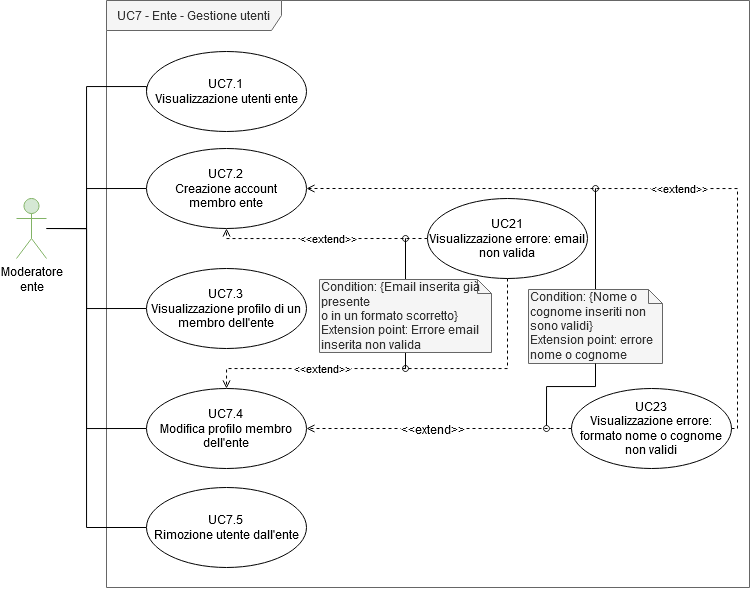
\includegraphics[scale=0.60]{res/images/uc7}
			\caption{Diagramma che riassume la gestione utenti appartenenti a un ente nella web app.}
		\end{figure}

		\begin{itemize}
			\item \textbf{Attori Primari}: Moderatore ente.
			\item \textbf{Descrizione}: L'utente può gestire gli utenti del proprio ente, eseguendo modifiche e cancellazioni di account esistenti o aggiunte di nuovi account.
			\item \textbf{Precondizione}: L'utente è autenticato e naviga nella gestione utenti per l'ente associato.
			\item \textbf{Postcondizione}: L'utente ha visualizzato o gestito gli utenti appartenenti al proprio ente.
			\item \textbf{Scenario Principale}:
			\begin{enumerate}
				\item{L'utente visualizza o gestisce gli utenti appartenenti al proprio ente.}
			\end{enumerate}	
		\end{itemize}
			
			\subsubsection{UC 7.1 - Visualizzazione utenti ente}
			\begin{itemize}
				\item \textbf{Attori Primari}: Moderatore ente.
				\item \textbf{Descrizione}: L'utente può visualizzare gli utenti del proprio ente.
				\item \textbf{Precondizione}: L'utente naviga nella gestione utenti per l'ente associato.
				\item \textbf{Postcondizione}: L'utente ha visualizzato la lista degli utenti appartenenti al proprio ente.
				\item \textbf{Scenario Principale}:
				\begin{enumerate}
					\item{L'utente visualizza la lista degli utenti appartenenti al proprio ente.}
				\end{enumerate}	
			\end{itemize}
			
			\subsubsection{UC 7.2 - Creazione account membro ente}
			\begin{itemize}
				\item \textbf{Attori Primari}: Moderatore ente.
				\item \textbf{Descrizione}: L'utente può creare un nuovo membro per il proprio ente.
				\item \textbf{Precondizione}: L'utente naviga nella gestione utenti per l'ente associato.
				\item \textbf{Postcondizione}: L'utente ha creato un nuovo account associato al proprio ente.
				\item \textbf{Scenario Principale}:
				\begin{enumerate}
					\item{L'utente deve compilare dei campi obbligatori per aggiungere un nuovo utente;}
					\item{L'utente compila il campo email (UC 7.2.1);}
					\item{L'utente compila il campo nome (UC 7.2.2);}
					\item{L'utente compila il campo cognome (UC 7.2.3);}
					\item{L'utente ha aggiunto un nuovo utente appartenente al proprio ente.}
				\end{enumerate}	
				\item \textbf{Estensioni}:
				\begin{itemize}
					\item L'utente inserisce un email non valida (UC 21)
					\item L'utente inserisce un nome o cognome non validi (UC 23)
				\end{itemize}
			\end{itemize}
			
			\paragraph{UC 7.2.1 - Inserimento email}
			\begin{itemize}
				\item \textbf{Attori Primari}: Moderatore ente.
				\item \textbf{Descrizione}: L'utente sta aggiungendo un nuovo utente e gli viene richiesto di compilare il campo obbligatorio per la email.
				\item \textbf{Precondizione}: L'utente sta compilando i campi richiesti per l'aggiunta di un nuovo utente.
				\item \textbf{Postcondizione}: L'utente ha compilato il campo richiesto per la creazione di un nuovo membro.
				\item \textbf{Scenario Principale}:
				\begin{enumerate}
					\item{L'utente ha compilato la email per il nuovo utente.}
				\end{enumerate}	
			\end{itemize}

			\paragraph{UC 7.2.2 - Inserimento nome}
			\begin{itemize}
				\item \textbf{Attori Primari}: Moderatore ente.
				\item \textbf{Descrizione}: L'utente sta aggiungendo un nuovo utente e gli viene richiesto di compilare il campo obbligatorio per il nome.
				\item \textbf{Precondizione}: L'utente sta compilando i campi richiesti per l'aggiunta di un nuovo utente.
				\item \textbf{Postcondizione}: L'utente ha compilato il campo richiesto per la creazione di un nuovo membro.
				\item \textbf{Scenario Principale}:
				\begin{enumerate}
					\item{L'utente ha compilato il nome per il nuovo utente.}
				\end{enumerate}	
			\end{itemize}

			\paragraph{UC 7.2.3 - Inserimento cognome}
			\begin{itemize}
				\item \textbf{Attori Primari}: Moderatore ente.
				\item \textbf{Descrizione}: L'utente sta aggiungendo un nuovo utente e gli viene richiesto di compilare il campo obbligatorio per il cognome.
				\item \textbf{Precondizione}: L'utente sta compilando i campi richiesti per l'aggiunta di un nuovo utente.
				\item \textbf{Postcondizione}: L'utente ha compilato il campo richiesto per la creazione di un nuovo membro.
				\item \textbf{Scenario Principale}:
				\begin{enumerate}
					\item{L'utente ha compilato il cognome per il nuovo utente.}
				\end{enumerate}	
			\end{itemize}

			\subsubsection{UC 7.3 - Visualizzazione profilo di un membro dell'ente}
			\begin{itemize}
				\item \textbf{Attori Primari}: Moderatore ente.
				\item \textbf{Descrizione}: L'utente può visualizzare i dati dell'utente selezionato dalla lista degli utenti del proprio ente.
				\item \textbf{Precondizione}: L'utente naviga nella gestione utenti per l'ente associato e visualizza i propri membri.
				\item \textbf{Postcondizione}: L'utente ha visualizzato i dati dell'utente selezionato appartenente al proprio ente.
				\item \textbf{Scenario Principale}:
				\begin{enumerate}
					\item{L'utente seleziona un utente dalla lista degli utenti del proprio ente;}
					\item{L'utente visualizza i dati dell'utente selezionato.}
				\end{enumerate}
			\end{itemize}


			\subsubsection{UC 7.4 - Modifica account membro ente}
			\begin{itemize}
				\item \textbf{Attori Primari}: Moderatore ente.
				\item \textbf{Descrizione}: L'utente può modificare un membro del proprio ente.
				\item \textbf{Precondizione}: L'utente naviga nella gestione utenti per l'ente associato.
				\item \textbf{Postcondizione}: L'utente ha modificato un nuovo account associato al proprio ente.
				\item \textbf{Scenario Principale}:
				\begin{enumerate}
					\item{L'utente deve compilare dei campi obbligatori per modificare un utente;}
					\item{L'utente compila il campo email (UC 7.4.1);}
					\item{L'utente compila il campo nome (UC 7.4.2);}
					\item{L'utente compila il campo cognome (UC 7.4.3);}
					\item{L'utente ha modificato un utente appartenente al proprio ente.}
				\end{enumerate}	
				\item \textbf{Estensioni}:
				\begin{itemize}
					\item L'utente inserisce un email non valida (UC 21)
					\item L'utente inserisce un nome o cognome non validi (UC 23)
				\end{itemize}
			\end{itemize}
			
			\paragraph{UC 7.4.1 - Modifica campo email}
			\begin{itemize}
				\item \textbf{Attori Primari}: Moderatore ente.
				\item \textbf{Descrizione}: L'utente sta modificando un utente e gli viene richiesto di compilare il campo obbligatorio per la email.
				\item \textbf{Precondizione}: L'utente sta compilando i campi richiesti per la modifica di un utente.
				\item \textbf{Postcondizione}: L'utente ha compilato il campo richiesto per la modifica di un membro.
				\item \textbf{Scenario Principale}:
				\begin{enumerate}
					\item{L'utente ha compilato la email dell'utente.}
				\end{enumerate}	
			\end{itemize}

			\paragraph{UC 7.4.2 - Modifica campo nome}
			\begin{itemize}
				\item \textbf{Attori Primari}: Moderatore ente.
				\item \textbf{Descrizione}: L'utente sta modificando un utente e gli viene richiesto di compilare il campo obbligatorio per il nome.
				\item \textbf{Precondizione}: L'utente sta compilando i campi richiesti per la modifica di un utente.
				\item \textbf{Postcondizione}: L'utente ha compilato il campo richiesto per la modifica di un membro.
				\item \textbf{Scenario Principale}:
				\begin{enumerate}
					\item{L'utente ha compilato il nome dell'utente.}
				\end{enumerate}	
			\end{itemize}

			\paragraph{UC 7.4.3 - Modifica campo cognome}
			\begin{itemize}
				\item \textbf{Attori Primari}: Moderatore ente.
				\item \textbf{Descrizione}: L'utente sta modificando un utente e gli viene richiesto di compilare il campo obbligatorio per il cognome.
				\item \textbf{Precondizione}: L'utente sta compilando i campi richiesti per la modifica di un utente.
				\item \textbf{Postcondizione}: L'utente ha compilato il campo richiesto per la modifica di un membro.
				\item \textbf{Scenario Principale}:
				\begin{enumerate}
					\item{L'utente ha compilato il cognome dell'utente.}
				\end{enumerate}	
			\end{itemize}

			
			\subsubsection{UC 7.5 - Rimozione utente dall'ente}
			\begin{itemize}
				\item \textbf{Attori Primari}: Moderatore ente.
				\item \textbf{Descrizione}: L'utente rimuove l'utente selezionato dalla lista degli utenti appartenenti al suo ente.
				\item \textbf{Precondizione}: L'utente naviga nella gestione utenti per l'ente associato e seleziona un utente.
				\item \textbf{Postcondizione}: L'utente ha rimosso l'utente selezionato appartenente al proprio ente.
				\item \textbf{Scenario Principale}:
				\begin{enumerate}
					\item{L'utente seleziona un utente appartenente al proprio ente da rimuovere;}
					\item{L'utente ha rimosso l'utente selezionato appartenente al proprio ente dal sistema.}
				\end{enumerate}		
			\end{itemize}
